\documentclass{article}

\usepackage{graphicx}
\usepackage[utf8]{inputenc}
\usepackage[T1]{fontenc}
\usepackage[portuguese]{babel}

\newcommand{\tit}[1]{\textit{#1}}

\begin{document}

\title{Gerador de FFT (Fast Fourier Transform) em Tempo Real}
\author{Esdras R. Carmo, Gabriel R. Hioki}

\maketitle
\newpage
\tableofcontents
\newpage

\section{Introdução}
A Transformada de Fourier Rápida (FFT) é um algoritmo que recebe um sinal
$x_n$ de amostras no domínio do tempo e retorna o vetor $X_m$ com os coeficientes
das funções senoidais em diferentes frequências. Em outras palavras, o FFT irá 
transformar um sinal no domínio do tempo para o domínio da frequência.

O FFT realiza otimizações no básico DFT (Discrete Fourier Transform) que consiste na seguinte
transformação linear:
$$
    X_m = \sum_{n=0}^{N-1}x_n w^{nm}
$$
onde $N$ é o tamanho dos vetores, $w = e^{2i\pi/N}$ são os fatores de rotação (\tit{twiddle}) e
$0 \leq m < N$. O algoritmo básico do somatório do DFT é feito usando $N^2$ operações, enquanto
o FFT consegue realizar o cálculo com $N \log N$ operações \cite{fft-hardware}.

\section{Diagrama de Blocos}

\begin{figure}[h!]
  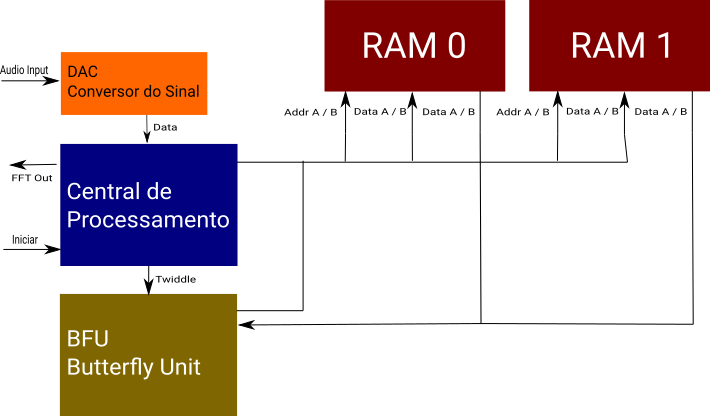
\includegraphics[width=\linewidth]{img/block-diagram.png}
  \caption{Diagrama de Blocos}
  \label{fig:diag}
\end{figure}

Descrição dos Blocos:
\begin{itemize}
    \item DAC / Conversor de Áudio: Hardware responsável por coletar o áudio em formato analógico
    e processar para um sinal digital;
    \item Central de Processamento (CP): Hardware responsável por escrever na RAM 0 o sinal digital e
    manipular os índices e prover o fator \tit{twiddle} para o BFU;
    \item Butterfly Unit (BFU): Hardware responsável por realizar as contas com os índices fornecidos
    pelo CP e gerar o resultado do FFT iterativamente na RAM 1;
    \item RAM 0 / 1: Duas unidades de memória com capacidade de leitura e escrita em dois endereços distintos.
    Capacidade para 32 palavras de memória de 16 bits.
\end{itemize}

\newpage
\bibliography{doc}
\bibliographystyle{ieeetr}
\end{document}
